\documentclass[10pt]{article}
\usepackage[a4paper,margin=18mm]{geometry}
\usepackage{amsmath,amssymb,booktabs,array,enumitem}
\usepackage[T1]{fontenc}\usepackage{lmodern}
\usepackage{tikz}\usetikzlibrary{shapes.gates.logic.US,positioning,arrows.meta,patterns,calc}
\usepackage[hidelinks]{hyperref}
\setlength{\parindent}{0pt}\setlength{\parskip}{4pt}
\setlength{\emergencystretch}{2em}
\newcommand{\VDD}{V_{DD}}
\newcommand{\mos}[4]{\begin{scope}[shift={(#1,#2)}]
\draw (0,.24)--(0,-.24);\draw (0,.20)--(.25,.20)--(.25,.5);
\draw (0,-.20)--(.25,-.20)--(.25,-.5);\draw (-.16,.23)--(-.16,-.23);
\ifnum#4=1\draw (-.26,0) circle (.06);\draw (-.75,0)--(-.32,0);\else\draw (-.75,0)--(-.16,0);\fi
\node[anchor=east,font=\scriptsize] at (-.76,0) {$#3$};\end{scope}}
\newcommand{\ground}[2]{\draw (#1,#2)--(#1,{#2-.12});\draw ({#1-.17},{#2-.12})--({#1+.17},{#2-.12});\draw ({#1-.11},{#2-.20})--({#1+.11},{#2-.20});}
\newcommand{\rail}[3]{\draw (#1,#2)--(#1,{#2+.14});\node[above,font=\scriptsize] at (#1,{#2+.14}) {$#3$};}

\newcommand{\hmos}[4]{\begin{scope}[shift={(#1,#2)}]
\draw(-.24,0)--(.24,0);\draw(-.2,0)--(-.2,-.25)--(-.5,-.25);\draw(.2,0)--(.2,-.25)--(.5,-.25);
\draw(-.23,.16)--(.23,.16);
\ifnum#4=1\draw(0,.26)circle(.06);\draw(0,.32)--(0,.75);\else\draw(0,.16)--(0,.75);\fi
\node[below,font=\scriptsize]at(0,-.32){#3};\end{scope}}
\begin{document}\begin{center}{\Large\bfseries 2010 Final -- Independently Corrected Solutions}\end{center}
\textbf{Scope.} All original Q1--Q8, totaling 130 printed points. The local 12-page answer PDF contains six graded booklets. Grades are comparison evidence, never a substitute for checking the original. Analog results use declared ideal models; no measured process result is claimed.
\textbf{1. Brief answers}
\begin{enumerate}[label=(\alph*),leftmargin=7mm]
\item Use common cell height and aligned $V_{DD}/V_{SS}$ rails for row abutment; use legal width increments and accessible signal pins while obeying the process design rules.
\item Capacitive external load power and internal-cell switching power (internal nodes), with their individual transition activities. This question says switching power; a separate short-circuit current contribution should not replace its internal-capacitance component.
\item Balance arrival times at reconvergent inputs; remove hazards with suitable logic factoring/consensus terms or suppress unnecessary transitions before they propagate. An output register limits downstream observation but does not eliminate energy already spent in preceding glitching gates.
\item Reduce package/supply inductance with short, wide paths and multiple power/ground pins; use local decoupling and control simultaneous-switching current/slew. Bounce follows $L\,di/dt$ plus resistive drop.
\item Charge sharing and leakage/noise sensitivity of a floating dynamic node. Direct same-phase dynamic cascades also risk irreversible false evaluation.
\item {\raggedright Ordinary N-domino implements noninverting cascades; evaluation inputs must obey the monotone rising/stable-input protocol. A dynamic node cannot recharge after a false discharge in the same evaluation phase.\par}
\item A core-limited die is sized mainly by internal logic/memory area; a pad-limited die is sized mainly by I/O pad perimeter/spacing requirements.
\item Convert the circuit/netlist into physical geometry: partition/floorplan, place cells, synthesize clock routes, route interconnect and verify physical/timing rules. Physical design is not the act of wafer fabrication.
\end{enumerate}
\textbf{2. The drawn low-cost register}
\begin{center}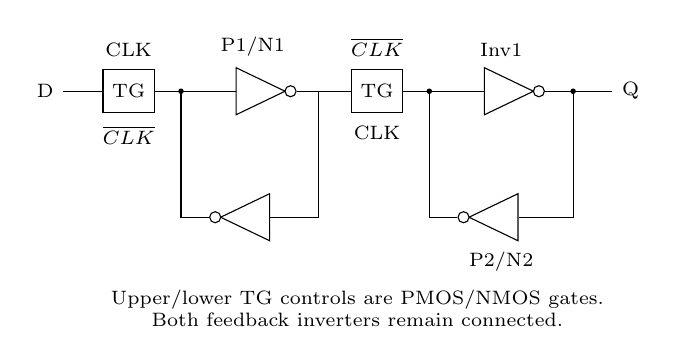
\begin{tikzpicture}[x=.83cm,y=.8cm,font=\scriptsize]
\node[draw,minimum width=.6cm,minimum height=.55cm](t1)at(.7,2.5){TG};\draw(-.3,2.5)node[left]{D}--(t1.west);\node[above]at(.7,2.9){CLK};\node[below]at(.7,2.1){$\overline{CLK}$};
\node[not gate US,draw,minimum width=.7cm](i1)at(2.6,2.5){};\draw(t1.east)--(i1.input);\node[above]at(2.6,2.9){P1/N1};\node[not gate US,draw,rotate=180,minimum width=.7cm](f1)at(2.6,.5){};\draw(i1.output)--(3.6,2.5)--(3.6,.5)--(f1.input);\draw(f1.output)--(1.5,.5)--(1.5,2.5);\fill(1.5,2.5)circle(1pt);
\node[draw,minimum width=.6cm,minimum height=.55cm](t2)at(4.5,2.5){TG};\draw(3.6,2.5)--(t2.west);\node[above]at(4.5,2.9){$\overline{CLK}$};\node[below]at(4.5,2.1){CLK};
\node[not gate US,draw,minimum width=.7cm](i2)at(6.4,2.5){};\draw(t2.east)--(i2.input);\node[above]at(6.4,2.9){Inv1};\draw(i2.output)--(8.1,2.5)node[right]{Q};\node[not gate US,draw,rotate=180,minimum width=.7cm](f2)at(6.4,.5){};\node[below]at(6.4,.1){P2/N2};\draw(7.5,2.5)--(7.5,.5)--(f2.input);\draw(f2.output)--(5.3,.5)--(5.3,2.5);\fill(5.3,2.5)circle(1pt);\fill(7.5,2.5)circle(1pt);\node[align=center]at(4.2,-.95){Upper/lower TG controls are PMOS/NMOS gates.\\Both feedback inverters remain connected.};\end{tikzpicture}\end{center}
The master TG has n-gate $\overline{CLK}$ / p-gate CLK, so it is transparent low; the slave n-gate CLK / p-gate $\overline{CLK}$ is transparent high. Two data inversions cancel: \textbf{a conditional positive-edge, noninverting register}. Always-connected feedback makes each half ratioed; transparency requires the input drive to overpower the old state. Complementary clocks require suitable transition/nonoverlap timing in a physical implementation.

For writing the slave input through its enabled TG, an old-high input is opposed by P2 and driven low by master N1. An old-low input is opposed by N2 and driven high by master P1. At the stated half-supply trip, sufficient divider inequalities are
\[\boxed{R_{P2}>R_{N1}+R_{TG,low},\qquad R_{N2}>R_{P1}+R_{TG,high}.}\]
In the explicitly ideal zero-resistance TG limit, these reduce to $R_{P2}>R_{N1}$ and $R_{N2}>R_{P1}$. The comparison is \emph{cross-device}, not pMOS against pMOS and nMOS against nMOS. Resistance scales inversely with each type's width; gate dimensions cannot be made numeric without drive/TG parameters. The master must likewise be writable by D. These inequalities test static write direction, not a specified write time.
\newpage
\textbf{3. Three complete transistor implementations}
Let $H=AB+\bar C(D+E)$, so $f=\bar H$. In a static network, parentheses are series and $\parallel$ is parallel. The following drawings explicitly label every physical gate/channel terminal.

\textbf{Dynamic: seven core MOS.} Precharge f high at CLK0; CLK1 enables the footer. The five-transistor PDN implements H. Stable evaluation inputs produce $f=\bar H$; the raw dynamic node has no restoring inverter.
\begin{center}\begin{tikzpicture}[x=.68cm,y=.68cm,font=\scriptsize]
\mos{0.0}{0.0}{\mathrm{CLK}}{1}
\draw(0.25,0.5)--(0.25,0.75)node[above]{$ V_{DD} $};
\draw(0.25,-0.5)--(0.25,-0.75)node[below]{$ f $};
\node[right]at(0.55,0.0){Ppre};
\mos{4.8}{0.0}{A}{0}
\draw(5.05,0.5)--(5.05,0.75)node[above]{$ f $};
\draw(5.05,-0.5)--(5.05,-0.75)node[below]{$ u $};
\node[right]at(5.35,0.0){NA};
\mos{9.6}{0.0}{B}{0}
\draw(9.85,0.5)--(9.85,0.75)node[above]{$ u $};
\draw(9.85,-0.5)--(9.85,-0.75)node[below]{$ e $};
\node[right]at(10.15,0.0){NB};
\mos{14.399999999999999}{0.0}{\bar C}{0}
\draw(14.649999999999999,0.5)--(14.649999999999999,0.75)node[above]{$ f $};
\draw(14.649999999999999,-0.5)--(14.649999999999999,-0.75)node[below]{$ v $};
\node[right]at(14.95,0.0){NC};
\mos{0.0}{-2.8}{D}{0}
\draw(0.25,-2.3)--(0.25,-2.05)node[above]{$ v $};
\draw(0.25,-3.3)--(0.25,-3.55)node[below]{$ e $};
\node[right]at(0.55,-2.8){ND};
\mos{4.8}{-2.8}{E}{0}
\draw(5.05,-2.3)--(5.05,-2.05)node[above]{$ v $};
\draw(5.05,-3.3)--(5.05,-3.55)node[below]{$ e $};
\node[right]at(5.35,-2.8){NE};
\mos{9.6}{-2.8}{\mathrm{CLK}}{0}
\draw(9.85,-2.3)--(9.85,-2.05)node[above]{$ e $};
\draw(9.85,-3.3)--(9.85,-3.55)node[below]{$ 0 $};
\node[right]at(10.15,-2.8){Nclk};
\end{tikzpicture}\\\small Dynamic core; add the C-complement inverter shown below. Equal terminal names denote connected wires. nMOS bodies use GND, pMOS bodies $V_{DD}$.\end{center}\begin{center}\begin{tikzpicture}[x=.68cm,y=.68cm,font=\scriptsize]
\mos{0.0}{0.0}{C}{1}
\draw(0.25,0.5)--(0.25,0.75)node[above]{$ V_{DD} $};
\draw(0.25,-0.5)--(0.25,-0.75)node[below]{$ \bar C $};
\node[right]at(0.55,0.0){CinvP};
\mos{4.8}{0.0}{C}{0}
\draw(5.05,0.5)--(5.05,0.75)node[above]{$ \bar C $};
\draw(5.05,-0.5)--(5.05,-0.75)node[below]{$ 0 $};
\node[right]at(5.35,0.0){CinvN};
\end{tikzpicture}\\\small Local complement generation for dynamic/static cores. Equal terminal names denote connected wires. nMOS bodies use GND, pMOS bodies $V_{DD}$.\end{center}
This is 9 MOS including local $\bar C$. Hold-state leakage/charge sharing and the monotonic input condition remain relevant.

\textbf{Fully differential: twelve core MOS.} The f PDN implements H; the $\bar f$ PDN implements $(\bar A+\bar B)(C+\bar D\bar E)=\bar H$. Cross-coupled pMOS loads restore the opposite output. Exactly one PDN conducts for all 32 input words.
\begin{center}\begin{tikzpicture}[x=.68cm,y=.68cm,font=\scriptsize]
\mos{0.0}{0.0}{\bar f}{1}
\draw(0.25,0.5)--(0.25,0.75)node[above]{$ V_{DD} $};
\draw(0.25,-0.5)--(0.25,-0.75)node[below]{$ f $};
\node[right]at(0.55,0.0){Pf};
\mos{4.8}{0.0}{f}{1}
\draw(5.05,0.5)--(5.05,0.75)node[above]{$ V_{DD} $};
\draw(5.05,-0.5)--(5.05,-0.75)node[below]{$ \bar f $};
\node[right]at(5.35,0.0){Pg};
\mos{9.6}{0.0}{A}{0}
\draw(9.85,0.5)--(9.85,0.75)node[above]{$ f $};
\draw(9.85,-0.5)--(9.85,-0.75)node[below]{$ u $};
\node[right]at(10.15,0.0){NA};
\mos{14.399999999999999}{0.0}{B}{0}
\draw(14.649999999999999,0.5)--(14.649999999999999,0.75)node[above]{$ u $};
\draw(14.649999999999999,-0.5)--(14.649999999999999,-0.75)node[below]{$ 0 $};
\node[right]at(14.95,0.0){NB};
\mos{0.0}{-2.8}{\bar C}{0}
\draw(0.25,-2.3)--(0.25,-2.05)node[above]{$ f $};
\draw(0.25,-3.3)--(0.25,-3.55)node[below]{$ v $};
\node[right]at(0.55,-2.8){NC};
\mos{4.8}{-2.8}{D}{0}
\draw(5.05,-2.3)--(5.05,-2.05)node[above]{$ v $};
\draw(5.05,-3.3)--(5.05,-3.55)node[below]{$ 0 $};
\node[right]at(5.35,-2.8){ND};
\mos{9.6}{-2.8}{E}{0}
\draw(9.85,-2.3)--(9.85,-2.05)node[above]{$ v $};
\draw(9.85,-3.3)--(9.85,-3.55)node[below]{$ 0 $};
\node[right]at(10.15,-2.8){NE};
\mos{14.399999999999999}{-2.8}{\bar A}{0}
\draw(14.649999999999999,-2.3)--(14.649999999999999,-2.05)node[above]{$ \bar f $};
\draw(14.649999999999999,-3.3)--(14.649999999999999,-3.55)node[below]{$ t $};
\node[right]at(14.95,-2.8){NAb};
\mos{0.0}{-5.6}{\bar B}{0}
\draw(0.25,-5.1)--(0.25,-4.85)node[above]{$ \bar f $};
\draw(0.25,-6.1)--(0.25,-6.35)node[below]{$ t $};
\node[right]at(0.55,-5.6){NBb};
\mos{4.8}{-5.6}{C}{0}
\draw(5.05,-5.1)--(5.05,-4.85)node[above]{$ t $};
\draw(5.05,-6.1)--(5.05,-6.35)node[below]{$ 0 $};
\node[right]at(5.35,-5.6){NCt};
\mos{9.6}{-5.6}{\bar D}{0}
\draw(9.85,-5.1)--(9.85,-4.85)node[above]{$ t $};
\draw(9.85,-6.1)--(9.85,-6.35)node[below]{$ j $};
\node[right]at(10.15,-5.6){NDb};
\mos{14.399999999999999}{-5.6}{\bar E}{0}
\draw(14.649999999999999,-5.1)--(14.649999999999999,-4.85)node[above]{$ j $};
\draw(14.649999999999999,-6.1)--(14.649999999999999,-6.35)node[below]{$ 0 $};
\node[right]at(14.95,-5.6){NEb};
\end{tikzpicture}\\\small DCVSL core; f is the original required output. Equal terminal names denote connected wires. nMOS bodies use GND, pMOS bodies $V_{DD}$.\end{center}
\newpage\textbf{Fully differential complement generators.} If only true primary inputs are available, generate all five complements, adding 10 MOS for a total of 22. The core itself assumes these full-rail complementary inputs, not floating gate terminals.
\begin{center}\begin{tikzpicture}[x=.68cm,y=.68cm,font=\scriptsize]
\mos{0.0}{0.0}{A}{1}
\draw(0.25,0.5)--(0.25,0.75)node[above]{$ V_{DD} $};
\draw(0.25,-0.5)--(0.25,-0.75)node[below]{$ \bar A $};
\node[right]at(0.55,0.0){AinvP};
\mos{4.8}{0.0}{A}{0}
\draw(5.05,0.5)--(5.05,0.75)node[above]{$ \bar A $};
\draw(5.05,-0.5)--(5.05,-0.75)node[below]{$ 0 $};
\node[right]at(5.35,0.0){AinvN};
\mos{9.6}{0.0}{B}{1}
\draw(9.85,0.5)--(9.85,0.75)node[above]{$ V_{DD} $};
\draw(9.85,-0.5)--(9.85,-0.75)node[below]{$ \bar B $};
\node[right]at(10.15,0.0){BinvP};
\mos{14.399999999999999}{0.0}{B}{0}
\draw(14.649999999999999,0.5)--(14.649999999999999,0.75)node[above]{$ \bar B $};
\draw(14.649999999999999,-0.5)--(14.649999999999999,-0.75)node[below]{$ 0 $};
\node[right]at(14.95,0.0){BinvN};
\mos{0.0}{-2.8}{C}{1}
\draw(0.25,-2.3)--(0.25,-2.05)node[above]{$ V_{DD} $};
\draw(0.25,-3.3)--(0.25,-3.55)node[below]{$ \bar C $};
\node[right]at(0.55,-2.8){CinvP};
\mos{4.8}{-2.8}{C}{0}
\draw(5.05,-2.3)--(5.05,-2.05)node[above]{$ \bar C $};
\draw(5.05,-3.3)--(5.05,-3.55)node[below]{$ 0 $};
\node[right]at(5.35,-2.8){CinvN};
\mos{9.6}{-2.8}{D}{1}
\draw(9.85,-2.3)--(9.85,-2.05)node[above]{$ V_{DD} $};
\draw(9.85,-3.3)--(9.85,-3.55)node[below]{$ \bar D $};
\node[right]at(10.15,-2.8){DinvP};
\mos{14.399999999999999}{-2.8}{D}{0}
\draw(14.649999999999999,-2.3)--(14.649999999999999,-2.05)node[above]{$ \bar D $};
\draw(14.649999999999999,-3.3)--(14.649999999999999,-3.55)node[below]{$ 0 $};
\node[right]at(14.95,-2.8){DinvN};
\mos{0.0}{-5.6}{E}{1}
\draw(0.25,-5.1)--(0.25,-4.85)node[above]{$ V_{DD} $};
\draw(0.25,-6.1)--(0.25,-6.35)node[below]{$ \bar E $};
\node[right]at(0.55,-5.6){EinvP};
\mos{4.8}{-5.6}{E}{0}
\draw(5.05,-5.1)--(5.05,-4.85)node[above]{$ \bar E $};
\draw(5.05,-6.1)--(5.05,-6.35)node[below]{$ 0 $};
\node[right]at(5.35,-5.6){EinvN};
\end{tikzpicture}\\\small All five complementary inputs. Equal terminal names denote connected wires. nMOS bodies use GND, pMOS bodies $V_{DD}$.\end{center}
\textbf{Static CMOS: ten core MOS, twelve including the C inverter.} The PDN is $AB\parallel[\bar C(D\parallel E)]$. Its pMOS dual is $(A\parallel B)[\bar C\parallel(DE)]$; because pMOS turns on for a low gate, its conduction condition is precisely $\bar H$.
\begin{center}\begin{tikzpicture}[x=.68cm,y=.68cm,font=\scriptsize]
\mos{0.0}{0.0}{A}{1}
\draw(0.25,0.5)--(0.25,0.75)node[above]{$ V_{DD} $};
\draw(0.25,-0.5)--(0.25,-0.75)node[below]{$ p $};
\node[right]at(0.55,0.0){PA};
\mos{4.8}{0.0}{B}{1}
\draw(5.05,0.5)--(5.05,0.75)node[above]{$ V_{DD} $};
\draw(5.05,-0.5)--(5.05,-0.75)node[below]{$ p $};
\node[right]at(5.35,0.0){PB};
\mos{9.6}{0.0}{\bar C}{1}
\draw(9.85,0.5)--(9.85,0.75)node[above]{$ p $};
\draw(9.85,-0.5)--(9.85,-0.75)node[below]{$ f $};
\node[right]at(10.15,0.0){PC};
\mos{14.399999999999999}{0.0}{D}{1}
\draw(14.649999999999999,0.5)--(14.649999999999999,0.75)node[above]{$ p $};
\draw(14.649999999999999,-0.5)--(14.649999999999999,-0.75)node[below]{$ q $};
\node[right]at(14.95,0.0){PD};
\mos{0.0}{-2.8}{E}{1}
\draw(0.25,-2.3)--(0.25,-2.05)node[above]{$ q $};
\draw(0.25,-3.3)--(0.25,-3.55)node[below]{$ f $};
\node[right]at(0.55,-2.8){PE};
\mos{4.8}{-2.8}{A}{0}
\draw(5.05,-2.3)--(5.05,-2.05)node[above]{$ f $};
\draw(5.05,-3.3)--(5.05,-3.55)node[below]{$ u $};
\node[right]at(5.35,-2.8){NA};
\mos{9.6}{-2.8}{B}{0}
\draw(9.85,-2.3)--(9.85,-2.05)node[above]{$ u $};
\draw(9.85,-3.3)--(9.85,-3.55)node[below]{$ 0 $};
\node[right]at(10.15,-2.8){NB};
\mos{14.399999999999999}{-2.8}{\bar C}{0}
\draw(14.649999999999999,-2.3)--(14.649999999999999,-2.05)node[above]{$ f $};
\draw(14.649999999999999,-3.3)--(14.649999999999999,-3.55)node[below]{$ v $};
\node[right]at(14.95,-2.8){NC};
\mos{0.0}{-5.6}{D}{0}
\draw(0.25,-5.1)--(0.25,-4.85)node[above]{$ v $};
\draw(0.25,-6.1)--(0.25,-6.35)node[below]{$ 0 $};
\node[right]at(0.55,-5.6){ND};
\mos{4.8}{-5.6}{E}{0}
\draw(5.05,-5.1)--(5.05,-4.85)node[above]{$ v $};
\draw(5.05,-6.1)--(5.05,-6.35)node[below]{$ 0 $};
\node[right]at(5.35,-5.6){NE};
\end{tikzpicture}\\\small Complementary static core; C inverter already shown. No clock. Equal terminal names denote connected wires. nMOS bodies use GND, pMOS bodies $V_{DD}$.\end{center}
Do not attach an output inverter to these cores without also changing the required polarity. The saved graph checks all 32 Boolean inputs with exclusive pullup/pulldown conduction, and both dynamic phases.
\newpage
\textbf{4. Balanced dynamic sizing and the impossible clock-power target}
\begin{center}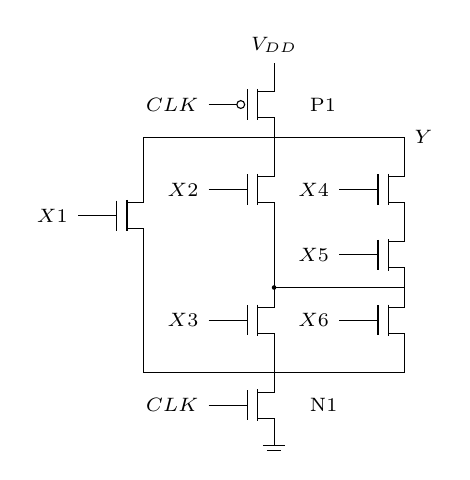
\begin{tikzpicture}[scale=.83,font=\scriptsize]
\mos{2}{5.5}{CLK}{1}\rail{2.25}{6}{V_{DD}}\node[right]at(2.65,5.5){P1};\draw(.25,5)--(4.25,5)node[right]{$Y$};
\mos{0}{3.8}{X1}{0}\draw(.25,4.3)--(.25,5);\draw(.25,3.3)--(.25,1.4);
\mos{2}{4.2}{X2}{0}\draw(2.25,4.7)--(2.25,5);\draw(2.25,3.7)--(2.25,2.7);
\mos{4}{4.2}{X4}{0}\mos{4}{3.2}{X5}{0}\draw(4.25,4.7)--(4.25,5);\draw(2.25,2.7)--(4.25,2.7);\fill(2.25,2.7)circle(1pt);
\mos{2}{2.2}{X3}{0}\mos{4}{2.2}{X6}{0}\draw(.25,1.4)--(4.25,1.4);\draw(2.25,1.7)--(2.25,1.4);\draw(4.25,1.7)--(4.25,1.4);
\mos{2}{.9}{CLK}{0}\ground{2.25}{.4}\node[right]at(2.65,.9){N1};
\end{tikzpicture}\\Figure 2: A dynamic logic circuit.\end{center}
The five minimal discharge paths are X1--N1, X2--X3--N1, X2--X6--N1, X4--X5--X3--N1, X4--X5--X6--N1. The two bottom X3/X6 branches are parallel, not two independent whole trees.

Let $R_P$ be P1's ON resistance. At common $L=.18\,\mu$m and $\mu_n=2\mu_p$, an nMOS of width $W$ has $R_N/R_P=2/W$ for $W$ in $\mu$m. Matching all minimal paths to $R_P$ matches the \emph{worst} fall time to rise time; parallel simultaneous conduction makes some fall times faster.

One simple valid sizing is
\begin{center}\begin{tabular}{cccccccc}\toprule Device&X1&X2&X3&X4&X5&X6&N1\\\midrule
$W\;(\mu m)$&4&8&8&16&16&8&4\\
$R_N/R_P$&$1/2$&$1/4$&$1/4$&$1/8$&$1/8$&$1/4$&$1/2$\\\bottomrule\end{tabular}\end{center}
All lengths remain $.18\,\mu$m. For a general family, let $q=R_{N1}/R_P$ and $a=R_{X2}/R_P$, with $0<q<1$, $0<a<1-q$. Then
\[R_{X1}/R_P=1-q,\quad R_{X3}/R_P=R_{X6}/R_P=1-q-a,\quad R_{X4}/R_P=R_{X5}/R_P=a/2.\]
Convert each ratio r to width $W=2/r\;\mu$m. Internal diffusion loads are excluded by this elementary matching model.

(b) The clock drives P1 and N1. P1 alone has capacitance C; N1 capacitance is $(W_{N1}/4)C$. Therefore
\[P_{clk}=fCV_{DD}^2(1+W_{N1}/4)<1.5fCV_{DD}^2\quad\Longrightarrow\quad W_{N1}<2\,\mu m.\]
But any finite balanced path must have $R_{N1}<R_P$, which requires $W_{N1}>2\,\mu m$. \textbf{No finite positive sizing satisfies both requirements.} Even the equality limit $W_{N1}=2$ consumes exactly $1.5fCV_{DD}^2$ and leaves no resistance budget for the functional devices. Scaling P1 would alter a fixed premise. A graded student size cannot override this contradiction.
\newpage
\textbf{5. NP timing and correct sharing-only states}
\begin{center}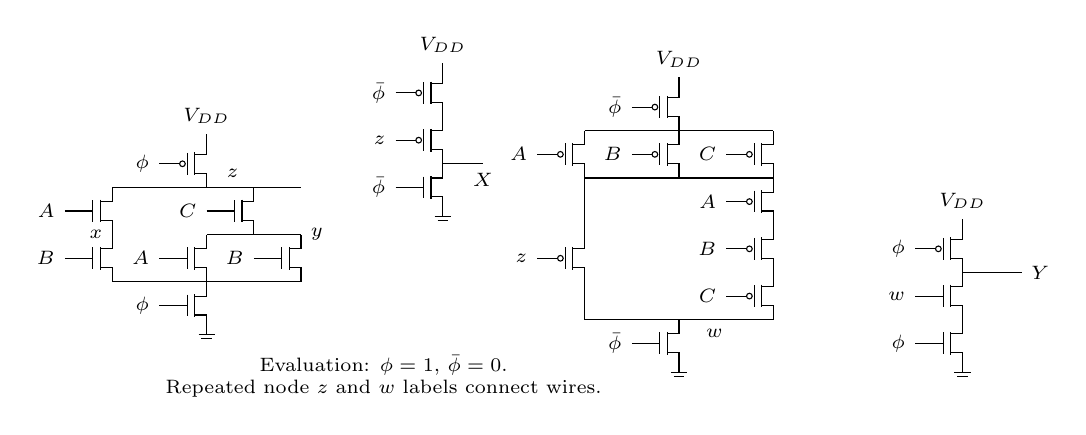
\begin{tikzpicture}[scale=.60,font=\scriptsize]
\mos{2}{5.8}{\phi}{1}\rail{2.25}{6.3}{V_{DD}}\draw(.25,5.3)--(4.25,5.3);\node[above]at(2.8,5.3){$z$};
\mos{0}{4.8}{A}{0}\mos{0}{3.8}{B}{0}\node[left]at(.25,4.3){$x$};\mos{3}{4.8}{C}{0}\draw(3.25,4.3)--(4.25,4.3);\mos{2}{3.8}{A}{0}\mos{4}{3.8}{B}{0}\draw(2.25,4.3)--(3.25,4.3);\node[right]at(4.25,4.3){$y$};\draw(.25,3.3)--(4.25,3.3);\mos{2}{2.8}{\phi}{0}\ground{2.25}{2.3}
\mos{7}{7.3}{\bar\phi}{1}\rail{7.25}{7.8}{V_{DD}}\mos{7}{6.3}{z}{1}\mos{7}{5.3}{\bar\phi}{0}\ground{7.25}{4.8}\draw(7.25,5.8)--(8.1,5.8)node[below]{$X$};
\mos{12}{7}{\bar\phi}{1}\rail{12.25}{7.5}{V_{DD}}\draw(10.25,6.5)--(14.25,6.5);\mos{10}{6}{A}{1}\mos{12}{6}{B}{1}\mos{14}{6}{C}{1}\draw(10.25,5.5)--(14.25,5.5);
\mos{10}{3.8}{z}{1}\draw(10.25,4.3)--(10.25,5.5);\draw(10.25,3.3)--(10.25,2.5)--(14.25,2.5);
\mos{14}{5}{A}{1}\mos{14}{4}{B}{1}\mos{14}{3}{C}{1}\mos{12}{2}{\bar\phi}{0}\ground{12.25}{1.5}\node[below]at(13,2.5){$w$};
\mos{18}{4}{\phi}{1}\rail{18.25}{4.5}{V_{DD}}\mos{18}{3}{w}{0}\mos{18}{2}{\phi}{0}\ground{18.25}{1.5}\draw(18.25,3.5)--(19.5,3.5)node[right]{$Y$};
\node[align=center]at(6,1.3){Evaluation: $\phi=1$, $\bar\phi=0$.\\Repeated node $z$ and $w$ labels connect wires.};\end{tikzpicture}\end{center}
During evaluation, $z=\overline{AB+AC+BC}$, X is majority, and Y is three-input parity. The middle p-dynamic node w rises for 000 or exactly two ones. The z device is below the three parallel pMOS inputs, so it is not a branch directly bypassing them. The final gate is clocked; w drives only its one nMOS input.

The z load is $4C$ (one X p-gate and one middle p-gate), and the w load is $C$. Output X/Y loads are not supplied and drain capacitance is explicitly ignored. Keep symbolic external loads $C_X,C_Y$ before taking that ideal limit.
\begin{center}\begin{tabular}{p{58mm}p{50mm}}\toprule Reachable path&Source-defined average delay\\\midrule
inputs $\to z\to X$, 111&$40RC/7+3RC_X/2$\\
inputs $\to z\to X$, exactly two ones&$8RC+3RC_X/2$\\
primary inputs $\to w\to Y$, 000&$8RC/3+3RC_Y/2$\\
inputs $\to z\to w\to Y$, exactly two ones&$10RC+3RC_Y/2$\\\bottomrule\end{tabular}\end{center}
For z discharge, 111 gives $R+(2R\parallel1.5R)=13R/7$; two ones give $3R$. Its precharge resistance is $R$. For w, 000 gives $R+R/3+3R=13R/3$, while two ones give $3R$; reset resistance is $R$. Thus w's mean delay is $8RC/3$ or $2RC$. A z-driven w transition requires two ones, so $8RC$ and $2RC$ sensitize together. Combining independent extrema from incompatible words does not establish a physical path. Under the printed mean-delay metric and $C_X=C_Y=0$,
\[\boxed{t_{cd}=8RC/3,\qquad t_{pd}=10RC.}\]
This is the source's averaged delay abstraction, not a measured minimum/maximum transient bound. The zero final-stage RC is the unloaded/parasitic-neglected limit, not instantaneous physical switching. Evaluation inputs must settle/obey monotonicity; arbitrary input races are outside this estimate.

(b) A sharing-only case must have no actual ground path. With z precharged to 1.8 V and internal nodes initially zero, 001 connects only y to z:
\[V_z=1.8\frac{2}{2+.8}=\frac97\,V\simeq1.2857V.\]
For 100, only x joins z, giving 1.5 V. Both exceed the pMOS turn-on boundary $1.8-.6=1.2$ V; 010 does not connect either internal capacitor to z. Therefore \textbf{the specified ideal sharing test is safe}, with a small $1/7$-V worst margin to pMOS enable. Pooling both x and y is invalid: A=C=1 opens a real majority discharge path. This conclusion uses the 2010 values; another year's smaller $C_z$ or different threshold would change the test. Leakage, charge injection, finite evaluation time and noise are not quantified by this test.
\newpage
\textbf{6. Signed skew, setup and hold}
Define $\delta=t_{capture}-t_{launch}$. Setup at $T=10$ ns requires
\[t_{pd,logic}\le10-.8-1.6+\delta=7.6+\delta.\]
The printed .1 ns does not give a sign. For a skew magnitude bounded by .1 ns, the guarantee is$\boxed{t_{pd,logic}\le7.5 ns}$; capture late by .1 ns would allow 7.7 ns. Hold is
\[.4+t_{cd,logic}\ge1.2+\delta.\]
On the direct R2--R3 path, assuming the printed .2/.3 ns wire/buffer delays are also their minimum delays, $n$ noninverting buffers give
\[.4+.2+.3n\ge1.2+.1\quad\Longrightarrow\quad n\ge3.\]
Two suffice only for nominal zero/early capture skew. Three buffers guarantee the stated magnitude case and give setup requirement $.8+.2+.9+1.6=3.5ns$, safely below 9.9 ns. Retain R1--R2's7.5 ns logic bound.
\begin{center}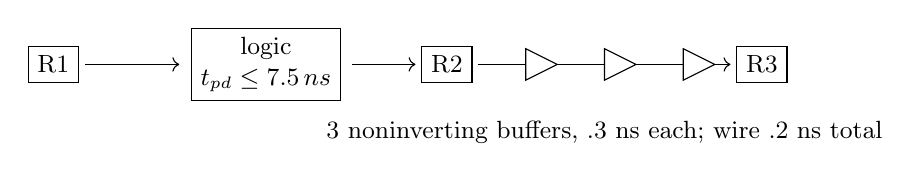
\begin{tikzpicture}[font=\small]
\node[draw]at(0,0){R1};\node[draw,align=center]at(2.7,0){logic\\$t_{pd}\le7.5\,ns$};\node[draw]at(5,0){R2};\node[draw]at(9,0){R3};\draw[->](.4,0)--(1.6,0);\draw[->](3.8,0)--(4.6,0);\draw(5.4,0)--(6,0);\foreach\x in{6,7,8}{\draw(\x,-.2)--(\x,.2)--(\x+.4,0)--cycle;}\draw(6.4,0)--(7,0) (7.4,0)--(8,0);\draw[->](8.4,0)--(8.6,0);\node[below]at(7,-.6){3 noninverting buffers, .3 ns each; wire .2 ns total};
\end{tikzpicture}\end{center}
All three registers retain the original common clock; the added buffers are on the data path. For a physical guarantee, use actual contamination delays: $t_{ccq}+t_{cd,wire}+\sum t_{cd,buf}\ge t_{hold}+\delta$. Propagation delay alone does not certify hold. The numerical three-buffer answer uses the explicitly declared single-delay classroom convention.
\newpage\textbf{7. Literal sixteen-MOS layout extraction}
\begin{center}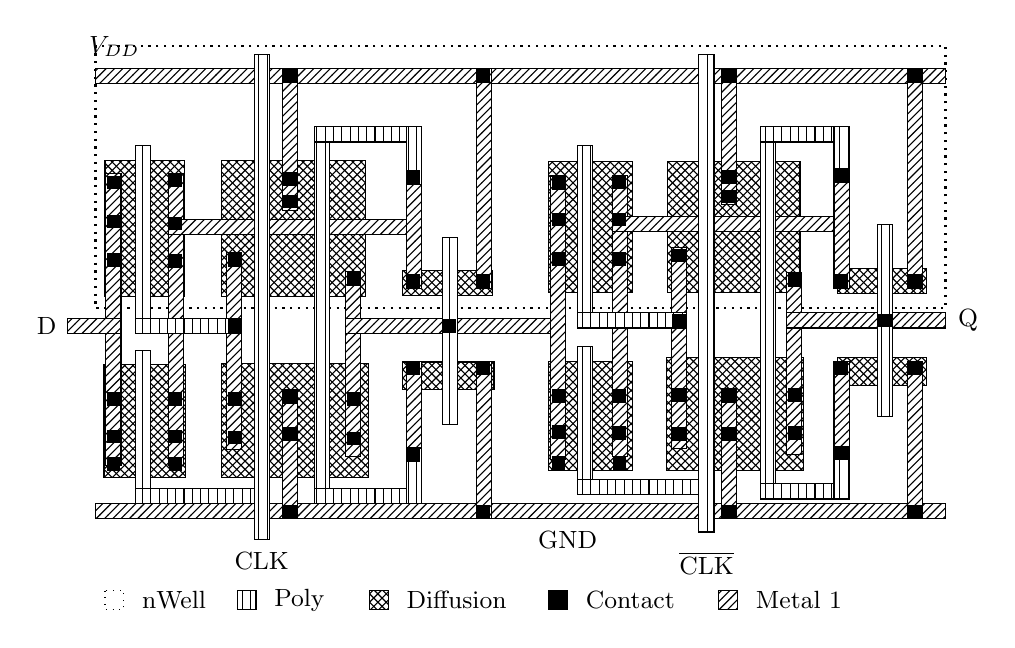
\begin{tikzpicture}[x=.012cm,y=-.012cm,font=\small]
\tikzset{lm/.style={preaction={fill=white},pattern=north east lines,pattern color=black},ld/.style={preaction={fill=white},pattern=crosshatch,pattern color=black},lp/.style={preaction={fill=white},pattern=vertical lines,pattern color=black}}
\draw[dotted,thick](400,108)rectangle(1300,386);
\draw[ld](410,230)rectangle(494,374);
\draw[ld](533,230)rectangle(686,374);
\draw[ld](725,346)rectangle(820,373);
\draw[ld](880,231)rectangle(969,369);
\draw[ld](1006,231)rectangle(1146,369);
\draw[ld](1186,344)rectangle(1280,370);
\draw[ld](409,446)rectangle(495,565);
\draw[ld](533,445)rectangle(689,565);
\draw[ld](725,443)rectangle(822,472);
\draw[ld](880,442)rectangle(969,558);
\draw[ld](1005,438)rectangle(1150,558);
\draw[ld](1186,438)rectangle(1280,468);
\draw[lm](400,132.0)rectangle(1300,148.0);
\draw[lm](400,593.0)rectangle(1300,609.0);
\draw[lm](411.0,243.0)rectangle(427.0,553.0);
\draw[lm](477.0,243.0)rectangle(493.0,553.0);
\draw[lm](477.0,292.0)rectangle(745.0,308.0);
\draw[lm](729.0,239.0)rectangle(745.0,365.0);
\draw[lm](539.0,327.0)rectangle(555.0,536.0);
\draw[lm](598.0,132.0)rectangle(614.0,283.0);
\draw[lm](598.0,472.0)rectangle(614.0,609.0);
\draw[lm](665.0,347.0)rectangle(681.0,543.0);
\draw[lm](665.0,397.0)rectangle(898.0,413.0);
\draw[lm](803.0,132.0)rectangle(819.0,365.0);
\draw[lm](803.0,442.0)rectangle(819.0,609.0);
\draw[lm](729.0,442.0)rectangle(745.0,550.0);
\draw[lm](882.0,246.0)rectangle(898.0,546.0);
\draw[lm](947.0,245.0)rectangle(963.0,543.0);
\draw[lm](947.0,289.0)rectangle(1198.0,305.0);
\draw[lm](1182.0,237.0)rectangle(1198.0,365.0);
\draw[lm](1010.0,322.0)rectangle(1026.0,535.0);
\draw[lm](1063.0,132.0)rectangle(1079.0,276.0);
\draw[lm](1063.0,471.0)rectangle(1079.0,609.0);
\draw[lm](1132.0,348.0)rectangle(1148.0,541.0);
\draw[lm](1132.0,391.0)rectangle(1300,407.0);
\draw[lm](1260.0,132.0)rectangle(1276.0,365.0);
\draw[lm](1260.0,442.0)rectangle(1276.0,609.0);
\draw[lm](1182.0,442.0)rectangle(1198.0,548.0);
\draw[lp](442.0,214.0)rectangle(458.0,413.0);
\draw[lp](442.0,397.0)rectangle(555.0,413.0);
\draw[lp](442.0,431.0)rectangle(458.0,593.0);
\draw[lp](442.0,577.0)rectangle(584.0,593.0);
\draw[lp](568.0,117.0)rectangle(584.0,631.0);
\draw[lp](632.0,194.0)rectangle(648.0,593.0);
\draw[lp](632.0,194.0)rectangle(745.0,210.0);
\draw[lp](729.0,194.0)rectangle(745.0,255.0);
\draw[lp](632.0,577.0)rectangle(745.0,593.0);
\draw[lp](729.0,534.0)rectangle(745.0,593.0);
\draw[lp](767.0,311.0)rectangle(783.0,509.0);
\draw[lp](910.0,214.0)rectangle(926.0,407.0);
\draw[lp](910.0,391.0)rectangle(1026.0,407.0);
\draw[lp](910.0,427.0)rectangle(926.0,583.0);
\draw[lp](910.0,567.0)rectangle(1055.0,583.0);
\draw[lp](1039.0,117.0)rectangle(1055.0,623.0);
\draw[lp](1104.0,194.0)rectangle(1120.0,588.0);
\draw[lp](1104.0,194.0)rectangle(1198.0,210.0);
\draw[lp](1182.0,194.0)rectangle(1198.0,253.0);
\draw[lp](1104.0,572.0)rectangle(1198.0,588.0);
\draw[lp](1182.0,532.0)rectangle(1198.0,588.0);
\draw[lp](1228.0,297.0)rectangle(1244.0,501.0);
\draw[fill=black](540.5,398.5)rectangle(553.5,411.5);
\draw[fill=black](730.5,240.5)rectangle(743.5,253.5);
\draw[fill=black](730.5,535.5)rectangle(743.5,548.5);
\draw[fill=black](768.5,398.5)rectangle(781.5,411.5);
\draw[fill=black](1011.5,392.5)rectangle(1024.5,405.5);
\draw[fill=black](1183.5,238.5)rectangle(1196.5,251.5);
\draw[fill=black](1183.5,533.5)rectangle(1196.5,546.5);
\draw[fill=black](1229.5,392.5)rectangle(1242.5,405.5);
\draw[fill=black](599.5,133.5)rectangle(612.5,146.5);
\draw[fill=black](599.5,594.5)rectangle(612.5,607.5);
\draw[fill=black](804.5,133.5)rectangle(817.5,146.5);
\draw[fill=black](804.5,594.5)rectangle(817.5,607.5);
\draw[fill=black](1064.5,133.5)rectangle(1077.5,146.5);
\draw[fill=black](1064.5,594.5)rectangle(1077.5,607.5);
\draw[fill=black](1261.5,133.5)rectangle(1274.5,146.5);
\draw[fill=black](1261.5,594.5)rectangle(1274.5,607.5);
\draw[fill=black](412.5,246.5)rectangle(425.5,259.5);
\draw[fill=black](412.5,287.5)rectangle(425.5,300.5);
\draw[fill=black](412.5,328.5)rectangle(425.5,341.5);
\draw[fill=black](478.5,244.5)rectangle(491.5,257.5);
\draw[fill=black](478.5,289.5)rectangle(491.5,302.5);
\draw[fill=black](478.5,329.5)rectangle(491.5,342.5);
\draw[fill=black](540.5,328.5)rectangle(553.5,341.5);
\draw[fill=black](599.5,242.5)rectangle(612.5,255.5);
\draw[fill=black](599.5,266.5)rectangle(612.5,279.5);
\draw[fill=black](666.5,348.5)rectangle(679.5,361.5);
\draw[fill=black](730.5,350.5)rectangle(743.5,363.5);
\draw[fill=black](804.5,350.5)rectangle(817.5,363.5);
\draw[fill=black](883.5,247.5)rectangle(896.5,260.5);
\draw[fill=black](883.5,285.5)rectangle(896.5,298.5);
\draw[fill=black](883.5,327.5)rectangle(896.5,340.5);
\draw[fill=black](948.5,246.5)rectangle(961.5,259.5);
\draw[fill=black](948.5,285.5)rectangle(961.5,298.5);
\draw[fill=black](948.5,327.5)rectangle(961.5,340.5);
\draw[fill=black](1011.5,323.5)rectangle(1024.5,336.5);
\draw[fill=black](1064.5,240.5)rectangle(1077.5,253.5);
\draw[fill=black](1064.5,261.5)rectangle(1077.5,274.5);
\draw[fill=black](1133.5,349.5)rectangle(1146.5,362.5);
\draw[fill=black](1183.5,350.5)rectangle(1196.5,363.5);
\draw[fill=black](1261.5,350.5)rectangle(1274.5,363.5);
\draw[fill=black](412.5,475.5)rectangle(425.5,488.5);
\draw[fill=black](412.5,515.5)rectangle(425.5,528.5);
\draw[fill=black](412.5,544.5)rectangle(425.5,557.5);
\draw[fill=black](478.5,475.5)rectangle(491.5,488.5);
\draw[fill=black](478.5,515.5)rectangle(491.5,528.5);
\draw[fill=black](478.5,544.5)rectangle(491.5,557.5);
\draw[fill=black](540.5,475.5)rectangle(553.5,488.5);
\draw[fill=black](540.5,516.5)rectangle(553.5,529.5);
\draw[fill=black](599.5,473.5)rectangle(612.5,486.5);
\draw[fill=black](599.5,512.5)rectangle(612.5,525.5);
\draw[fill=black](666.5,475.5)rectangle(679.5,488.5);
\draw[fill=black](666.5,517.5)rectangle(679.5,530.5);
\draw[fill=black](730.5,443.5)rectangle(743.5,456.5);
\draw[fill=black](804.5,443.5)rectangle(817.5,456.5);
\draw[fill=black](883.5,472.5)rectangle(896.5,485.5);
\draw[fill=black](883.5,510.5)rectangle(896.5,523.5);
\draw[fill=black](883.5,543.5)rectangle(896.5,556.5);
\draw[fill=black](948.5,472.5)rectangle(961.5,485.5);
\draw[fill=black](948.5,511.5)rectangle(961.5,524.5);
\draw[fill=black](948.5,543.5)rectangle(961.5,556.5);
\draw[fill=black](1011.5,471.5)rectangle(1024.5,484.5);
\draw[fill=black](1011.5,512.5)rectangle(1024.5,525.5);
\draw[fill=black](1064.5,472.5)rectangle(1077.5,485.5);
\draw[fill=black](1064.5,512.5)rectangle(1077.5,525.5);
\draw[fill=black](1133.5,471.5)rectangle(1146.5,484.5);
\draw[fill=black](1133.5,511.5)rectangle(1146.5,524.5);
\draw[fill=black](1183.5,443.5)rectangle(1196.5,456.5);
\draw[fill=black](1261.5,443.5)rectangle(1274.5,456.5);
\node[above]at(420,130){$V_{DD}$};\node[below]at(900,612){GND};\draw[lm](370,397)rectangle(427,413);
\node[left]at(369,405){D};\node[right]at(1303,399){Q};
\node[below]at(576,634){CLK};\node[below]at(1047,634){$\overline{\mathrm{CLK}}$};
\draw[dotted](410,685)rectangle(430,705);\node[right]at(439,695){nWell};
\draw[lp](550,685)rectangle(570,705);\node[right]at(579,695){Poly};
\draw[ld](690,685)rectangle(710,705);\node[right]at(719,695){Diffusion};
\draw[fill=black](880,685)rectangle(900,705);\node[right]at(909,695){Contact};
\draw[lm](1060,685)rectangle(1080,705);\node[right]at(1089,695){Metal 1};
\end{tikzpicture}\\[2mm]\small Geometry normalized; all eight physical gate columns and contacts retained.\end{center}\begin{center}\begin{tikzpicture}[x=.68cm,y=.68cm,font=\scriptsize]
\mos{0.0}{0.0}{\mathrm{c1}}{1}
\draw(0.25,0.5)--(0.25,0.75)node[above]{$ D $};
\draw(0.25,-0.5)--(0.25,-0.75)node[below]{$ b $};
\node[right]at(0.55,0.0){P1};
\mos{4.8}{0.0}{\mathrm{CLK}}{0}
\draw(5.05,0.5)--(5.05,0.75)node[above]{$ D $};
\draw(5.05,-0.5)--(5.05,-0.75)node[below]{$ b $};
\node[right]at(5.35,0.0){N1};
\mos{9.6}{0.0}{\mathrm{CLK}}{1}
\draw(9.85,0.5)--(9.85,0.75)node[above]{$ V_{DD} $};
\draw(9.85,-0.5)--(9.85,-0.75)node[below]{$ \mathrm{c1} $};
\node[right]at(10.15,0.0){P2};
\mos{14.399999999999999}{0.0}{\mathrm{CLK}}{0}
\draw(14.649999999999999,0.5)--(14.649999999999999,0.75)node[above]{$ \mathrm{c1} $};
\draw(14.649999999999999,-0.5)--(14.649999999999999,-0.75)node[below]{$ 0 $};
\node[right]at(14.95,0.0){N2};
\mos{0.0}{-2.8}{b}{1}
\draw(0.25,-2.3)--(0.25,-2.05)node[above]{$ V_{DD} $};
\draw(0.25,-3.3)--(0.25,-3.55)node[below]{$ m $};
\node[right]at(0.55,-2.8){P3};
\mos{4.8}{-2.8}{b}{0}
\draw(5.05,-2.3)--(5.05,-2.05)node[above]{$ m $};
\draw(5.05,-3.3)--(5.05,-3.55)node[below]{$ 0 $};
\node[right]at(5.35,-2.8){N3};
\mos{9.6}{-2.8}{m}{1}
\draw(9.85,-2.3)--(9.85,-2.05)node[above]{$ V_{DD} $};
\draw(9.85,-3.3)--(9.85,-3.55)node[below]{$ b $};
\node[right]at(10.15,-2.8){P4};
\mos{14.399999999999999}{-2.8}{m}{0}
\draw(14.649999999999999,-2.3)--(14.649999999999999,-2.05)node[above]{$ b $};
\draw(14.649999999999999,-3.3)--(14.649999999999999,-3.55)node[below]{$ 0 $};
\node[right]at(14.95,-2.8){N4};
\mos{0.0}{-5.6}{\mathrm{c2}}{1}
\draw(0.25,-5.1)--(0.25,-4.85)node[above]{$ m $};
\draw(0.25,-6.1)--(0.25,-6.35)node[below]{$ s $};
\node[right]at(0.55,-5.6){P5};
\mos{4.8}{-5.6}{\overline{\mathrm{CLK}}}{0}
\draw(5.05,-5.1)--(5.05,-4.85)node[above]{$ m $};
\draw(5.05,-6.1)--(5.05,-6.35)node[below]{$ s $};
\node[right]at(5.35,-5.6){N5};
\mos{9.6}{-5.6}{\overline{\mathrm{CLK}}}{1}
\draw(9.85,-5.1)--(9.85,-4.85)node[above]{$ V_{DD} $};
\draw(9.85,-6.1)--(9.85,-6.35)node[below]{$ \mathrm{c2} $};
\node[right]at(10.15,-5.6){P6};
\mos{14.399999999999999}{-5.6}{\overline{\mathrm{CLK}}}{0}
\draw(14.649999999999999,-5.1)--(14.649999999999999,-4.85)node[above]{$ \mathrm{c2} $};
\draw(14.649999999999999,-6.1)--(14.649999999999999,-6.35)node[below]{$ 0 $};
\node[right]at(14.95,-5.6){N6};
\mos{0.0}{-8.399999999999999}{s}{1}
\draw(0.25,-7.899999999999999)--(0.25,-7.649999999999999)node[above]{$ V_{DD} $};
\draw(0.25,-8.899999999999999)--(0.25,-9.149999999999999)node[below]{$ Q $};
\node[right]at(0.55,-8.399999999999999){P7};
\mos{4.8}{-8.399999999999999}{s}{0}
\draw(5.05,-7.899999999999999)--(5.05,-7.649999999999999)node[above]{$ Q $};
\draw(5.05,-8.899999999999999)--(5.05,-9.149999999999999)node[below]{$ 0 $};
\node[right]at(5.35,-8.399999999999999){N7};
\mos{9.6}{-8.399999999999999}{Q}{1}
\draw(9.85,-7.899999999999999)--(9.85,-7.649999999999999)node[above]{$ V_{DD} $};
\draw(9.85,-8.899999999999999)--(9.85,-9.149999999999999)node[below]{$ s $};
\node[right]at(10.15,-8.399999999999999){P8};
\mos{14.399999999999999}{-8.399999999999999}{Q}{0}
\draw(14.649999999999999,-7.899999999999999)--(14.649999999999999,-7.649999999999999)node[above]{$ s $};
\draw(14.649999999999999,-8.899999999999999)--(14.649999999999999,-9.149999999999999)node[below]{$ 0 $};
\node[right]at(14.95,-8.399999999999999){N8};
\end{tikzpicture}\\\small Eight physical columns, 16 MOS; all local clock inverters and always-connected feedback preserved. Equal terminal names denote connected wires. nMOS bodies use GND, pMOS bodies $V_{DD}$.\end{center}
The first device pair is a TG whose channel starts at D. Master: TG D$\leftrightarrow$b enabled at CLK=1; clock inverter CLK$\to$c1; storage inverter b$\to$m; fixed feedback inverter m$\to$b. Slave: TG m$\leftrightarrow$s enabled at CLK=0; clock inverter CLKB$\to$c2; storage inverter s$\to$Q; fixed feedback inverter Q$\to$s. The 16 physical MOS count follows four crossings per row per half. No outer input/output inverters exist in this original.

With sufficient write drive, the master follows while CLK is high and holds at the falling edge; the slave then passes that stored word. Two data inversions cancel, so the conditional circuit is a \textbf{negative-edge, noninverting register}. Its clock polarity differs from the positive-edge Figure 1 in Q2. Keep each source's clock routing. Feedback remains connected during writing and can oppose new data, so the original without sizes does not prove writeability or settling. Replacing it with a two-TG latch would change its electrical connections.
\newpage
\textbf{8. Upper Schmitt trip: use the given voltage and bias-dependent currents}
\begin{center}\begin{tikzpicture}[scale=.82,font=\scriptsize]
\mos{1}{4.5}{}{1}\mos{1}{3.5}{}{1}\mos{1}{2}{}{0}\mos{1}{1}{}{0}\rail{1.25}{5}{1.8\,V}\ground{1.25}{.5}
\foreach\y/\name in{4.5/P1,3.5/P2,2/N2,1/N1}{\node[right]at(1.5,\y){\name};}
\draw(1.25,2.5)--(1.25,3);\draw(1.25,2.75)--(5,2.75)node[right]{$V_{out}$};\draw(-.8,1)--(-.8,4.5);\foreach\y in{1,2,3.5,4.5}{\draw(-.8,\y)--(.25,\y);}\node[left]at(-.8,2.75){$V_{in}$};
\hmos{3.2}{4.25}{P3}{1}\draw(1.25,4)--(2.7,4);\draw(3.7,4)--(4.2,4);\ground{4.2}{4}\draw(3.2,5)--(4.6,5)--(4.6,2.75);
\hmos{3.2}{1.75}{N3}{0}\draw(1.25,1.5)--(2.7,1.5);\draw(3.7,1.5)--(4.2,1.5);\rail{4.2}{1.5}{1.8\,V}\draw(3.2,2.5)--(3.2,2.75);\fill(3.2,2.75)circle(1pt);
\begin{scope}[xshift=7cm]\draw[->](0,0)--(4.5,0)node[right]{$V_{in}$};\draw[->](0,0)--(0,3.5)node[above]{$V_{out}$};\draw plot[smooth]coordinates{(0,3)(1,3)(1.4,2.8)(1.65,1.5)(1.9,.2)(3.5,0)};\draw plot[smooth]coordinates{(0,3)(2,3)(2.8,2.8)(3,1.5)(3.2,.2)(3.7,0)};\draw[->](.5,3)--(1,3);\draw[->](3,1.8)--(3,1.2);\draw[->](1.65,1.2)--(1.65,1.8);\draw[->](2.8,.01)--(2.3,.01);\draw[dashed](1.65,0)--(1.65,1.5) (3,0)--(3,1.5);\node[below]at(1.65,0){$V_T^-$};\node[below]at(3,0){$V_T^+=1.2$};\end{scope}
\end{tikzpicture}\\Figure 6: Schmitt circuit and qualitative VTC.\end{center}
The original explicitly states $V_T^+=1.2$ V. Just before the rising trip, $V_{out}\simeq V_{DD}$ keeps N3 on. N2 begins conduction when internal node a satisfies $V_a=V_T^+-V_{tn}=.6$ V. Neglect body effect/channel-length modulation and use the standard long-channel model. N1 is at the saturation boundary with overdrive .6 V; N3 has gate 1.8 V, source .6 V, drain 1.8 V and saturation overdrive .6 V. Current balance is
\[\frac{\beta_{N1}}2(1.2-.6)^2=\frac{\beta_{N3}}2(1.8-1.2)^2,
\qquad\boxed{\beta_{N1}/\beta_{N3}=1}.\]
Treating both ON resistances as bias independent and inverting a divider ratio can instead produce 2; that is not a valid beta extraction. The devices have different gate/source biases, so resistance cannot be inferred as a common constant times the inverse of beta. At this onset, their equal currents coexist with $V_{DS,N1}=.6$ V and $V_{DS,N3}=1.2$ V: therefore $R_{N3}=2R_{N1}$ is consistent with \emph{equal beta}. The different bias coefficients explain why a resistance ratio of two does not imply a beta ratio of two. A full switching point including the pMOS network/body effect would need extra parameters; the expression above is the threshold-onset sizing approximation with its assumptions visible.

\textbf{Sources and checks.} The original Fall 2010 prompt governs every premise. All 12 student PDF pages were compared locally; identity fields are not redistributed. Saved standard-library graph checks cover 32 logic words, two dynamic phases, 64 dynamic-gate inputs, 16 literal-layout settled/contention states, and exact path/clock/share/skew constraints. Reference mechanisms are checked against the instructor's \href{https://www.ee.ncu.edu.tw/jfli/public_html/VLSI/lecture/ch04.pdf}{CMOS electrical characteristics}, \href{https://www.ee.ncu.edu.tw/jfli/public_html/VLSI/lecture/ch06.pdf}{advanced logic} and \href{https://www.ee.ncu.edu.tw/jfli/public_html/VLSI/lecture/ch07.pdf}{sequential circuits}. No grader's score is correctness proof.\end{document}